\rfcnumber{0005}
\rfctitle{Proof of Relay}
\rfcdate{October 2025}
\rfcauthor{Lukas Pohanka (@NumberFour8), Qianchen Yu (@QYuQianchen)}
\section{RFC-0005: Proof of Relay}\label{rfc-0005-proof-of-relay}

\begin{itemize}
\tightlist
\item
  \textbf{RFC Number:} 0005
\item
  \textbf{Title:} Proof of Relay
\item
  \textbf{Status:} Finalised
\item
  \textbf{Author(s):} Lukas Pohanka (@NumberFour8), Qianchen Yu
  (@QYuQianchen)
\item
  \textbf{Created:} 2025-04-02
\item
  \textbf{Updated:} 2025-10-27
\item
  \textbf{Version:} v1.0.0 (Finalised)
\item
  \textbf{Supersedes:} none
\item
  \textbf{Related Links:}
  \href{../RFC-0002-mixnet-keywords/0002-mixnet-keywords.md}{RFC-0002},
  \href{../RFC-0004-hopr-packet-protocol/0004-hopr-packet-protocol.md}{RFC-0004}
\end{itemize}

\subsection{1. Abstract}\label{abstract}

This RFC describes the structures and protocol for establishing a Proof
of Relay (PoR) for HOPR packets sent between two peers via a relay node.
The PoR mechanism provides cryptographic proof that a relay node has
successfully delivered a packet to its destination, which can then be
used to claim payment for the relay service. This solves the fundamental
challenge of incentivising relay nodes in a trustless manner whilst
preserving sender anonymity.

\subsection{2. Motivation}\label{motivation}

The Proof of Relay mechanism addresses the challenge of ensuring
reliable packet delivery in a privacy-preserving mixnet with economic
incentives. When a sender (peer A) uses node B as a relay to deliver a
packet to destination node C, the mechanism establishes that:

\begin{enumerate}
\def\labelenumi{\arabic{enumi}.}
\tightlist
\item
  Node A has cryptographic guarantees that node B delivered A's packet
  to node C
\item
  After successful relaying to C, node B possesses a cryptographic proof
  of delivery
\item
  Node B can use this proof to claim a reward from node A through a
  payment channel
\item
  The identity of node A remains hidden from node C, preserving sender
  anonymity
\end{enumerate}

Without such a mechanism, relay nodes could claim payment without
actually forwarding packets, or senders would have to trust relay nodes
without verification. The PoR mechanism makes the payment conditional on
proof of actual relay service, creating a trustless,
incentive-compatible system.

\subsection{3. Terminology}\label{terminology}

The keywords ``MUST'', ``MUST NOT'', ``REQUIRED'', ``SHALL'', ``SHALL
NOT'', ``SHOULD'', ``SHOULD NOT'', ``RECOMMENDED'', ``MAY'', and
``OPTIONAL'' in this document are to be interpreted as described in
{[}01{]} when, and only when, they appear in all capitals, as shown
here.

All terminology used in this document, including general mix network
concepts and HOPR-specific definitions, is provided in
\href{../RFC-0002-mixnet-keywords/0002-mixnet-keywords.md}{RFC-0002}.
That document serves as the authoritative reference for the terminology
and conventions adopted across the HOPR RFC series. References to ``HOPR
packets'' or ``mixnet packets'' refer to a particular structure
(\codebubble{HOPR\_Packet}) defined in
\href{../RFC-0004-hopr-packet-protocol/0004-hopr-packet-protocol.md}{RFC-0004}.

In addition, this document defines the following proof-of-relay-specific
terms:

\begin{itemize}
\tightlist
\item
  \textbf{Channel} (or \textbf{Payment channel}): a unidirectional
  relation between two parties (source node and destination node) that
  holds a monetary balance. The source can pay out funds to the
  destination when certain conditions are met (specifically, when valid
  proof-of-relay tickets are presented).
\item
  \textbf{Ticket}: a cryptographic structure that enables probabilistic
  fund transfer within a payment channel. Tickets contain challenges
  that must be solved by the relay node to prove packet delivery.
\item
  \textbf{DomainSeparator}: a unique identifier that binds cryptographic
  signatures to a specific execution context (contract address, chain
  ID, etc.) to prevent replay attacks across different domains where the
  channel ledger may be deployed.
\item
  \textbf{Notice period (T\_closure)}: the minimum elapsed time required
  for an outgoing channel to transition from the
  \codebubble{PENDING\_TO\_CLOSE} state to the \codebubble{CLOSED}
  state. This period allows relay nodes to claim pending rewards before
  channel closure.
\end{itemize}

The above terms are formally defined in the following sections.

\subsubsection{3.1. Cryptographic and security
parameters}\label{cryptographic-and-security-parameters}

This document uses certain cryptographic and mathematical terms. A
security parameter \codebubble{L} is defined, and corresponding
cryptographic primitives are instantiated to achieve this security
level. The specific instantiation for the current version of this
protocol is provided in Appendix 1.

The security parameter \codebubble{L} SHALL NOT be less than 2\^{}128,
meaning the chosen cryptographic primitive instantiations SHALL provide
at least 128 bits of security against known attacks.

The following cryptographic primitives are required:

\begin{itemize}
\tightlist
\item
  \textbf{EC group}: a specific elliptic curve \codebubble{E} group over
  a finite field, where the computational Diffie-Hellman problem has
  hardness at least equal to the security parameter \codebubble{L}.
  Field elements are denoted using lowercase letters, whilst elliptic
  curve points (EC points) are denoted using uppercase letters.
\item
  \textbf{MUL(a,B)}: scalar multiplication of an EC point \codebubble{B}
  by a scalar \codebubble{a} from the corresponding finite field.
\item
  \textbf{ADD(A,B)}: addition of two EC points \codebubble{A} and
  \codebubble{B} on the elliptic curve.
\item
  \textbf{Public key}: a non-identity EC group element of large order,
  used to identify a node and establish shared secrets.
\item
  \textbf{Private key}: a scalar from the finite field of the chosen EC
  group, corresponding to a public key. Must be kept secret.
\item
  \textbf{Hash \codebubble{H(x)}}: a cryptographic hash function taking
  an input of any size and returning a fixed-length output. The security
  of \codebubble{H} against preimage, collision, and second-preimage
  attacks SHALL be at least \codebubble{L} bits.
\item
  \textbf{Verifiable random function (VRF)}: a function that produces a
  pseudo-random value along with a proof of correct computation. The
  output is publicly verifiable but cannot be forged or precomputed
  without the secret key.
\end{itemize}

Nodes and clients MUST implement handling for each of the above to
ensure compliance and fault tolerance within the HOPR PoR protocol.

The concrete choices of the above cryptographic primitives for the
implementation of version 1.0 are given in Appendix 1.

\subsection{4. Payment channels}\label{payment-channels}

Payment channels are the foundation of the HOPR incentive mechanism.
They enable efficient micropayments between nodes without requiring a
blockchain transaction for each packet relayed.

Let A, B, and C be peers participating in the mixnet. Each node
possesses its own private key (\codebubble{Kpriv\_A},
\codebubble{Kpriv\_B}, \codebubble{Kpriv\_C}) and the corresponding
public key (\codebubble{P\_A}, \codebubble{P\_B}, \codebubble{P\_C}).
Public keys are publicly exposed to enable packet routing and shared
secret establishment.

The public keys MUST be from an elliptic curve cryptosystem represented
by elliptic curve \codebubble{E}.

When node A wishes to communicate with node C using node B as a relay,
node A opens a unidirectional payment channel with node B (denoted A
-\textgreater{} B), depositing funds into this channel on-chain. The
channel holds the current balance and additional state information
shared between A and B, and funds flow strictly in the direction A
-\textgreater{} B.

MUST be strictly greater than 0 and strictly less than 2\^{}96 (to fit
within the ticket structure's amount field).

There MUST NOT be more than one payment channel between any two nodes A
and B in a given direction. Since channels are unidirectional, there MAY
simultaneously exist both a channel A -\textgreater{} B and a channel B
-\textgreater{} A.

Each channel has a unique, deterministic identifier: the channel ID. The
channel ID for A -\textgreater{} B MUST be computed as:
\codebubble{channel\_id = H(f(P\_A)||f(P\_B))} where \codebubble{||}
denotes byte-wise concatenation and \codebubble{f} represents a
deterministic encoding function for public keys (typically compressed EC
point encoding). This construction is directional: the source node's
public key appears first, followed by the destination node's public key.

Channels transition through three distinct lifecycle states:

\begin{enumerate}
\def\labelenumi{\arabic{enumi}.}
\tightlist
\item
  \textbf{OPEN}: the channel is active and can be used for packet relay
  payments
\item
  \textbf{PENDING\_TO\_CLOSE}: the channel is in the process of closing;
  nodes can still claim pending rewards during the notice period
\item
  \textbf{CLOSED}: the channel is permanently closed; no further
  operations are possible
\end{enumerate}

These states can be represented using the \codebubble{ChannelStatus}
enumeration:

\begin{codebubbleenv}
ChannelStatus { OPEN, PENDING_TO_CLOSE, CLOSED }
\end{codebubbleenv}

There is a structure called \codebubble{channel} that MUST contain at
least the following fields:

\begin{enumerate}
\def\labelenumi{\arabic{enumi}.}
\tightlist
\item
  \codebubble{source}: public key of the source node (A in this case)
\item
  \codebubble{destination}: public key of the destination node
  (beneficiary, B in this case)
\item
  \codebubble{balance} : an unsigned 96-bit integer
\item
  \codebubble{ticket\_index}: an unsigned 48-bit integer
\item
  \codebubble{channel\_epoch}: an unsigned 24-bit non-zero integer
\item
  \codebubble{status}: one of the \codebubble{ChannelStatus} values
\end{enumerate}

\begin{codebubbleenv}
Channel {
    source: [u8; |P_A|],
    destination: [u8; |P_B|],
    balance: u96,
    ticket_index: u48,
    channel_epoch: u24,
    status: ChannelStatus
}
\end{codebubbleenv}

Such structure is sufficient to describe the payment channel A
-\textgreater{} B.

Channels are uniquely identified by the \codebubble{channel\_id} above.
The fixed‑length byte string returned by the function is called
\codebubble{ChannelId}.

\subsubsection{4.1. Payment channel
life-cycle}\label{payment-channel-life-cycle}

A payment channel between nodes A -\textgreater{} B MUST always be
initiated by node A. It MUST be initialised with a non-zero
\codebubble{balance}, a \codebubble{ticket\_index} equal to
\codebubble{0}, \codebubble{channel\_epoch} equal to \codebubble{1} and
\codebubble{status} equal to \codebubble{Open}. To prevent spamming, the
funding \codebubble{balance} MUST be larger than
\codebubble{MIN\_USED\_BALANCE} and smaller than
\codebubble{MAX\_USED\_BALANCE}.

In such state, the node A is allowed to communicate with node C via B
and the node B can claim certain fixed amounts of \codebubble{balance}
to be paid out to it in return - as a reward for the relaying work. This
will be described in the later sections.

At any point in time, the channel initiator A can initiate a closure of
the channel A -\textgreater{} B. Such transition MUST change the
\codebubble{status} field to \codebubble{PENDING\_TO\_CLOSE} and this
change MUST be communicated to B. In such state, the node A MUST NOT be
allowed to communicate with C via B, but B MUST be allowed to still
claim any unclaimed rewards from the channel. However, B MUST NOT be
allowed to claim any rewards after \codebubble{T\_closure} has elapsed
since the transition to PENDING\_TO\_CLOSE. \codebubble{T\_closure} MUST
be measured in block timestamps, and both parties MUST derive it from
the same source.

After each claim is done by B, the \codebubble{ticket\_index} field MUST
be incremented by 1, and such change MUST be communicated to both A and
B. The increment MAY be done by an independent trusted third party
supervising the reward claims.

The initiator A SHALL transition the channel state to
\codebubble{CLOSED} (changing the \codebubble{status} to
\codebubble{CLOSED}). Such transition MUST NOT be possible before
\codebubble{T\_closure} has elapsed. The transition MUST be communicated
to B. In such state, the node A MUST NOT be allowed to communicate with
C via B, and B MUST NOT be allowed to claim any unclaimed rewards from
the channel. The \codebubble{balance} in the channel A -\textgreater{} B
MUST be reset to \codebubble{0} and its \codebubble{channel\_epoch} MUST
be incremented by \codebubble{1}.

At any point in time when the channel is at the state other than
\codebubble{CLOSED}, the channel destination B MAY unilaterally
transition the channel A -\textgreater{} B to state \codebubble{CLOSED}.
Node B SHALL claim unclaimed rewards before the state transition,
because any unclaimed rewards become unclaimable after the state
transition, resulting in a loss for node B. To prevent spamming, the
reward amount MUST be larger than \codebubble{MIN\_USED\_BALANCE} and
smaller than \codebubble{MAX\_USED\_BALANCE}.

\subsection{5. Tickets}\label{tickets}

Tickets are always created by a node that is the source (\codebubble{A})
of an existing channel. It is created whenever \codebubble{A} wishes to
send a HOPR packet to a certain destination (\codebubble{C}), while
having the existing channel's destination (\codebubble{B}) act as a
relay.

Their creation MAY happen at the same time as the HOPR packet, or MAY be
precomputed in advance when usage of a certain path is known beforehand.

A ticket:

\begin{enumerate}
\def\labelenumi{\arabic{enumi}.}
\tightlist
\item
  MUST be tied (via a cryptographic challenge) to a single HOPR packet
  (from
  \href{../RFC-0004-hopr-packet-protocol/0004-hopr-packet-protocol.md}{RFC-0004})
\item
  the cryptographic challenge MUST be solvable by the ticket recipient
  (\codebubble{B}) once it delivers the corresponding HOPR packet to
  \codebubble{C}
\item
  the solution of the cryptographic challenge MAY unlock a reward for
  ticket's recipient \codebubble{B} at expense of \codebubble{A}
\item
  MUST NOT contain information about packet's destination
  (\codebubble{C})
\end{enumerate}

\subsubsection{5.1. Ticket structure
encoding}\label{ticket-structure-encoding}

The ticket has the following structure:

\begin{codebubbleenv}
Ticket {
    channel_id: ChannelId,
    amount: u96,
    index: u48,
    index_offset: u32,
    encoded_win_prob: u56,
    channel_epoch: u24,
    challenge: ECPoint,
    signature: ECDSASignature
}
\end{codebubbleenv}

All multi-byte unsigned integers MUST use big-endian encoding when
serialised.

The \codebubble{ECPoint} is an encoding of an Elliptic curve point on
the chosen curve \codebubble{E} that corresponds to a cryptographic
challenge. Such challenge is later solved by the ticket recipient once
it forwards the attached packet to the next downstream node.

The encoding (for serialization) of the \codebubble{ECPoint} MUST be
unique and MAY be irreversible, in the sense that the original elliptic
point on the curve \codebubble{E} is not recoverable, but the encoding
uniquely identifies the said point.

The \codebubble{ECDSASignature} SHOULD use the
\href{https://eips.ethereum.org/EIPS/eip-2098}{ERC-2098 encoding}, the
public key recovery bit is stored in the most significant bit of the
\codebubble{s} value (which is guaranteed to be unused). Both
\codebubble{r} and \codebubble{s} use big-endian encoding when
serialised.

\begin{codebubbleenv}
ECDSASignature {
    r: u256
    s: u256
}
\end{codebubbleenv}

The ECDSA signature of the ticket MUST be computed over the
\href{https://eips.ethereum.org/EIPS/eip-712}{EIP‑712} hash
\codebubble{H\_ticket} of the \codebubble{ticket} typed-data using
\codebubble{domainSeparator} (\codebubble{dst}):

\begin{codebubbleenv}
H_1 = H(channel_id || amount || index || index_offset || channel_epoch || encoded_win_prob || challenge)
H_2 = H(0xfcb7796f00000000000000000000000000000000000000000000000000000000 || H_1)`
H_ticket = H(0x1901 || dst || H_2)
\end{codebubbleenv}

The \codebubble{ticket} signature MUST be done over the same elliptic
curve \codebubble{E} using the private key of the ticket creator
(issuer).

\subsubsection{5.2. Construction of Proof-of-Relay (PoR)
secrets}\label{construction-of-proof-of-relay-por-secrets}

This section uses terms defined in Section 2.2 in
\href{../RFC-0004-hopr-packet-protocol/0004-hopr-packet-protocol.md}{RFC-0004},
namely the \codebubble{SharedSecret\_i} generated for the
\codebubble{i}-th node on the path (\codebubble{i} ranges from 0 (sender
node) up to \codebubble{n} (destination node), i.e.~\codebubble{n} is
equal to the path length). Note that for 0-hop path (a direct packet
from sender to destination), \codebubble{n} = 1.

In the PoR mechanism, a cryptographic secret is established between
relay nodes and their adjacent nodes on the route.

Upon packet creation, the sender node creates two structures:

\begin{enumerate}
\def\labelenumi{\arabic{enumi}.}
\tightlist
\item
  the list of \codebubble{ProofOfRelayString\_i} for each
  \codebubble{i}-th node on the path for i \textgreater{} 0 up to
  \codebubble{n-1}. For \codebubble{n=1}, the list will be empty
\item
  the \codebubble{ProofOfRelayValues} structure
\end{enumerate}

Each \codebubble{ProofOfRelayString\_i} contains the
\codebubble{challenge} for the ticket for the \codebubble{i+1}-th node
and the \codebubble{hint} value for the same node. The \codebubble{hint}
value is later used by the \codebubble{i+1}-th node to validate that the
\codebubble{challenge} is not bogus, before it delivers the packet to
the next hop.

Due to this later verification, the \codebubble{hint} MUST use an
encoding useful for EC group computations on \codebubble{E} (here
denoted as \codebubble{RawECPoint}).

\begin{codebubbleenv}
ProofOfRelayString_i {
    challenge: ECPoint,
    hint: RawECPoint
}
\end{codebubbleenv}

The \codebubble{ProofOfRelayValues} structure contains the
\codebubble{challenge} and \codebubble{hint} to the first relayer on the
path, plus it MUST contain information about the path length. This
information is later used to set the correct price of the first ticket.

Path length MUST always be less than 4 (i.e.~maximum 3 hops).

\begin{codebubbleenv}
ProofOfRelayValues {
    challenge: ECPoint,
    hint: RawECPoint,
    path_len: u8
}
\end{codebubbleenv}

\paragraph{5.2.1. Creation of Proof of Relay strings and
values}\label{creation-of-proof-of-relay-strings-and-values}

Let \codebubble{HS} be the Hash to Field operation defined in
\href{../RFC-0004-hopr-packet-protocol/0004-hopr-packet-protocol.md}{RFC-0004}
over the field of the chosen \codebubble{E}.

The generation process of \codebubble{ProofOfRelayString\_i} proceeds as
follows for each \codebubble{i} from 0 to \codebubble{n-1}:

\begin{enumerate}
\def\labelenumi{\arabic{enumi}.}
\item
  The \codebubble{SharedKey\_i+1\_ack} is derived from the shared secret
  (\codebubble{SharedSecret\_i}) provided during the HOPR packet
  construction. \codebubble{SharedKey\_i+1\_ack} denotes the secret
  acknowledgement key for the next downstream node (\codebubble{i+1}).

  \begin{itemize}
  \tightlist
  \item
    if \codebubble{i} \textless{} \codebubble{n} :
    \codebubble{SharedKey\_i+1\_ack = HS(SharedKey\_i, "HASH\_KEY\_ACK\_KEY")}
  \item
    if \codebubble{i} = \codebubble{n} : the
    \codebubble{SharedKey\_i+1\_ack} MUST be generated as a uniformly
    random byte-string with the byte-length of \codebubble{E}'s field
    elements.
  \end{itemize}
\item
  The own shared secret \codebubble{SharedKey\_i\_own} from
  \codebubble{SharedSecret\_i} is generated as:
  \codebubble{SharedKey\_i\_own = HS(SharedKey\_i, "HASH\_KEY\_OWN\_KEY")}
\item
  The \codebubble{hint} value is computed:

  \begin{itemize}
  \tightlist
  \item
    if \codebubble{i} = 0:
    \codebubble{hint = HS(SharedKey\_0, "HASH\_KEY\_ACK\_KEY")}
  \item
    if \codebubble{i} \textgreater{} 0:
    \codebubble{hint = SharedKey\_i+1\_ack} (from step 1)
  \end{itemize}
\item
  For \codebubble{i} \textgreater{} 0, the
  \codebubble{ProofOfRelayString\_i} is composed and added to the list:

  \begin{itemize}
  \tightlist
  \item
    \codebubble{challenge} is computed as:
    \codebubble{challenge = MUL(SharedKey\_i\_own + SharedKey\_i+1\_ack, G)}
    and encoded as \codebubble{ECPoint}
  \item
    \codebubble{hint} is used from step 3.
  \end{itemize}
\item
  For \codebubble{i} = 0, the \codebubble{ProofOfRelayValues} is
  created:

  \begin{itemize}
  \tightlist
  \item
    \codebubble{challenge} is computed as:
    \codebubble{challenge = MUL(SharedKey\_i\_own + SharedKey\_i+1\_ack, G)}
    and encoded as \codebubble{ECPoint}
  \item
    \codebubble{hint} is used from step 3.
  \item
    \codebubble{path\_length} is set to \codebubble{n}
  \end{itemize}
\end{enumerate}

\subsubsection{5.3 Creation of the ticket for the first
relayer}\label{creation-of-the-ticket-for-the-first-relayer}

The first ticket MUST be created by the packet Sender and MUST contain
the \codebubble{challenge} field equal to the \codebubble{challenge} in
the \codebubble{ProofOfRelayValues} from the previous step.

\paragraph{\texorpdfstring{Multi-hop ticket: for \codebubble{n}
\textgreater{}
1}{Multi-hop ticket: for  \textgreater{} 1}}\label{multi-hop-ticket-for-n-1}

In this situation, the \codebubble{Channel} between the Sender and the
next hop MUST exist and be in the \codebubble{OPEN} state.

\begin{enumerate}
\def\labelenumi{\arabic{enumi}.}
\item
  The field \codebubble{channel\_id} MUST be set according to the
  \codebubble{Channel} leading from the Sender to the first packet
  relayer.
\item
  The \codebubble{amount} field SHOULD be set according to an expected
  packet price times the number of hops on the path (that is
  \codebubble{n} - 1).
\item
  The \codebubble{index} field MUST be set to the
  \codebubble{ticket\_index} + 1 from the corresponding
  \codebubble{Channel}.
\item
  The \codebubble{index\_offset} MUST be set to 1 in the current
  implementation.
\item
  The \codebubble{encoded\_win\_prob} SHOULD be set according to the
  expected ticket winning probability in the network.
\item
  The \codebubble{channel\_epoch} MUST be set to the
  \codebubble{channel\_epoch} from the corresponding
  \codebubble{Channel}.
\end{enumerate}

\paragraph{\texorpdfstring{Zero-hop ticket: \codebubble{n} =
1}{Zero-hop ticket:  = 1}}\label{zero-hop-ticket-n-1}

This is a specific case when the packet is 0-hop (\codebubble{n} = 1, it
is sent directly from the Sender to the Recipient). If the
\codebubble{Channel} between the Sender and Recipient does exist, it
MUST be ignored.

The \codebubble{Ticket} is still created:

\begin{enumerate}
\def\labelenumi{\arabic{enumi}.}
\item
  The \codebubble{channel\_id} MUST be set to
  \codebubble{H(P\_S || P\_R)} where \codebubble{P\_S} and
  \codebubble{P\_R} are public keys (or their encoding) of Sender and
  Recipient respectively.
\item
  The \codebubble{amount}, \codebubble{index} and
  \codebubble{channel\_epoch} MUST be 0
\item
  The \codebubble{index\_offset} MUST be 1
\item
  The \codebubble{encoded\_win\_prob} MUST be set to a value equivalent
  to the 0 winning probability
\end{enumerate}

In any case, once the \codebubble{Ticket} structure is complete, it MUST
be signed by the Sender, who MUST be always the first ticket's issuer.

As described in Section 2.5 in
\href{../RFC-0004-hopr-packet-protocol/0004-hopr-packet-protocol.md}{RFC-0004},
the complete encoded \codebubble{Ticket} structure becomes part of the
outgoing \codebubble{HOPR\_Packet}.

\subsubsection{5.4. Ticket processing at a
node}\label{ticket-processing-at-a-node}

This is inherently part of the packet processing from the
\href{../RFC-0004-hopr-packet-protocol/0004-hopr-packet-protocol.md}{RFC-0004}.
Once a node receives a \codebubble{HOPR\_Packet} structure, the
\codebubble{Ticket} is separated and its processing is a two-step
process:

\begin{enumerate}
\def\labelenumi{\arabic{enumi}.}
\tightlist
\item
  The ticket is pre-verified (this is already mentioned in section 4.4
  of RFC 0003).
\item
  If the packet is to be forwarded to a next node, the ticket MUST be
  fully-verified

  \begin{itemize}
  \tightlist
  \item
    If successful, the ticket is replaced with a new ticket in the
    \codebubble{HOPR\_Packet} for the next hop
  \end{itemize}
\end{enumerate}

\paragraph{5.4.1. Ticket
pre-verification}\label{ticket-pre-verification}

Failure to validate in any of the verification steps MUST result in
discarding the ticket and the corresponding \codebubble{HOPR\_Packet},
and interrupting the processing further.

If the extracted \codebubble{Ticket} structure cannot be deserialised,
the corresponding \codebubble{HOPR\_Packet} MUST be discarded. If the
\codebubble{Ticket} has been issued for an unknown channel, or it does
not correspond to the channel between the packet sender and the node
where it is being processed, or the channel is in the
\codebubble{CLOSED} state, the corresponding \codebubble{HOPR\_Packet}
MUST be discarded.

At this point, the node knows its \codebubble{SharedSecret\_i} with
which it is able to decrypt the \codebubble{HOPR\_Packet} and the
\codebubble{ProofOfRelayString\_i} has already been extracted from the
packet header (see section 4.2 in
\href{../RFC-0004-hopr-packet-protocol/0004-hopr-packet-protocol.md}{RFC-0004}).

\begin{enumerate}
\def\labelenumi{\arabic{enumi}.}
\tightlist
\item
  \codebubble{SharedSecret\_i} is used to derive
  \codebubble{SharedSecret\_i\_own} as per Section 4.2.1
\item
  The \codebubble{hint} is extracted from the
  \codebubble{ProofOfRelayString\_i}
\item
  Compute
  \codebubble{challenge\_check = ADD(SharedSecret\_i\_own, hint)}
\item
  The \codebubble{HOPR\_Packet} MUST be rejected if encoding of
  \codebubble{challenge\_check} does not match \codebubble{challenge}
  from the \codebubble{Ticket}
\end{enumerate}

If the pre-verification fails at any point, it still applies that the
discarded \codebubble{HOPR\_Packet} MUST be acknowledged (as per section
4.2.3.1).

\paragraph{5.4.2. Ticket validation and
replacement}\label{ticket-validation-and-replacement}

Let \codebubble{corr\_channel} be the \codebubble{Channel} that
corresponds to the \codebubble{channel\_id} on the \codebubble{Ticket}.
This channel MUST exist and not be in the \codebubble{CLOSED} state per
previous section, otherwise the entire \codebubble{HOPR\_Packet} has
been discarded.

If the packet is to be forwarded (as per section 4.3.1 in
\href{../RFC-0004-hopr-packet-protocol/0004-hopr-packet-protocol.md}{RFC-0004}),
the \codebubble{Ticket} MUST be verified as follows:

\begin{enumerate}
\def\labelenumi{\arabic{enumi}.}
\tightlist
\item
  the \codebubble{signature} of the \codebubble{Ticket} is verified - if
  the signature uses ERC-2098 encoding, the ticket issuer from the
  signature is recovered and compared to the public key of the packet
  sender (or its representation)
\item
  the \codebubble{amount} MUST be checked, so that it is greater than
  some given minimum ticket amount (this SHOULD be done with respect to
  the path position)
\item
  the \codebubble{channel\_epoch} on the \codebubble{Ticket} MUST be the
  current epoch of the \codebubble{corr\_channel}.
\item
  it MUST be checked that the packet sender has enough funds to cover
  the \codebubble{amount} of the ticket
\end{enumerate}

Once the above verifications have passed, verified ticket is stored as
\emph{unacknowledged} by the node and SHOULD be indexed by
\codebubble{hint}. The stored unacknowledged tickets are dealt with
later (see 4.2.3).

A new \codebubble{Ticket} for the packet forwarded to the next hop MUST
be created.

The \codebubble{HeaderPrefix} from the packet header contains the
current path position. This information is further used to determine
which type of ticket to create.

The path position is used to derive the number of remaining hops.

If the number of remaining hops is \textgreater{} 1, it MUST be checked
if a \codebubble{Channel} for the next hop exists from the current node,
and if it is in the \codebubble{OPEN} state. If not, the corresponding
\codebubble{HOPR\_Packet} is discarded and the process is interrupted.

The process of \codebubble{Ticket} creation from section 4.3 then
applies, either with the \codebubble{Channel} as the next hop channel in
a multi-hop ticket (if the number of remaining hops \textgreater{} 1),
or creates a zero-hop ticket if the number of remaining hops is 1.

The following applies in addition to 4.3:

\begin{itemize}
\tightlist
\item
  the \codebubble{amount} on the ticket in the multi-hop case MAY be
  adjusted (typically the \codebubble{amount} from the previous ticket
  is diminished by the packet price)
\item
  the \codebubble{challenge} MUST be set to \codebubble{challenge} from
  the \codebubble{ProofOfRelayString\_i} extracted from the
  \codebubble{HOPR\_Packet}
\end{itemize}

If the ticket validation fails at any point, it still applies that the
discarded \codebubble{HOPR\_Packet} MUST be acknowledged (as per section
4.2.3.1).

\paragraph{5.2.3. Ticket acknowledgement}\label{ticket-acknowledgement}

The following sections first describe how acknowledgements are created
when sent back to the original packet's sender, and secondly how a
received acknowledgement should be processed.

\subparagraph{5.2.3.1. Sending
acknowledgement}\label{sending-acknowledgement}

Per section 4.3.3 in
\href{../RFC-0004-hopr-packet-protocol/0004-hopr-packet-protocol.md}{RFC-0004},
each packet without \codebubble{NoAckFlag} set MUST be acknowledged.
Such an acknowledgement becomes a payload of a 0-hop packet sent from
the original packet's recipient to the original packet's sender.

\begin{codebubbleenv}
Acknowledgement {
    ack_secret: ECScalar,
    signature: ECDSASignature
}
\end{codebubbleenv}

There are two possibilities for how the \codebubble{ack\_secret} field
is calculated:

\begin{enumerate}
\def\labelenumi{\arabic{enumi}.}
\tightlist
\item
  if the \codebubble{HOPR\_Packet} being acknowledged has been
  successfully processed (along with a successfully validated ticket),
  the \codebubble{ack\_secret} MUST be calculated as:
\end{enumerate}

\codebubble{ack\_secret = HS(SharedSecret\_i, "HASH\_KEY\_ACK\_KEY")}

This EC field element MUST be encoded as a big-endian integer (denoted
as \codebubble{ECScalar}).

\begin{enumerate}
\def\labelenumi{\arabic{enumi}.}
\setcounter{enumi}{1}
\tightlist
\item
  if the processing of the \codebubble{HOPR\_Packet} failed for any
  reason (either failure of the packet processing in
  \href{../RFC-0004-hopr-packet-protocol/0004-hopr-packet-protocol.md}{RFC-0004}
  or during packet pre-verification or validation from Section 5.2):
  \codebubble{ack\_secret} is set to a random EC point on
  \codebubble{E}.
\end{enumerate}

The \codebubble{signature} field contains the signature of the encoded
\codebubble{ack\_secret} bytes. The signature is done over
\codebubble{H(ack\_secret)} using the private key of the acknowledging
party. For this purpose, the same EC cryptosystem for signing and
verification as with \codebubble{Ticket} SHOULD be used. The same
encoding MUST be used for the \codebubble{signature} field as for the
\codebubble{Ticket}.

\subparagraph{5.2.3.2. Receiving an
acknowledgement}\label{receiving-an-acknowledgement}

After the \codebubble{Ticket} has been extracted and validated by the
relay node, it awaits until the packet acknowledgement is received back
from the next hop. The node SHOULD discard tickets that haven't been
acknowledged for a certain given period of time.

Once an \codebubble{Acknowledgement} is received, the node MUST:

\begin{enumerate}
\def\labelenumi{\arabic{enumi}.}
\tightlist
\item
  validate the \codebubble{signature} of \codebubble{ack\_secret}. If
  invalid, the \codebubble{Acknowledgement} MUST be discarded.
\item
  decode \codebubble{ack\_secret} and calculate
  \codebubble{hint = MUL(ack\_secret, G)}
\end{enumerate}

The node then searches for a previously stored \emph{unacknowledged}
\codebubble{Ticket} with the corresponding \codebubble{hint} as index.

\begin{itemize}
\tightlist
\item
  If a \codebubble{Ticket} with corresponding \codebubble{hint} is
  found, it MUST be marked as \emph{acknowledged} and the
  \codebubble{ack\_secret} is then the missing part in the solution of
  the cryptographic challenge on that \codebubble{Ticket} (which
  corresponds to the packet that has just been acknowledged).
\end{itemize}

Let \codebubble{SharedSecret\_i\_own} be the value from 1) in Section
5.2.1. The \codebubble{response} to the \codebubble{Ticket} challenge
corresponding to the acknowledged packet is:

\codebubble{response = ack\_secret + SharedSecret\_i\_own}

The response is a field element of \codebubble{E}.

\begin{itemize}
\tightlist
\item
  If no matching \codebubble{Ticket} was found, the received
  \codebubble{Acknowledgement} SHOULD be discarded.
\end{itemize}

\subparagraph{5.2.3.3. Derivation of VRF parameters for an Acknowledged
ticket}\label{derivation-of-vrf-parameters-for-an-acknowledged-ticket}

Once the ticket becomes acknowledged, the node then calculates the
\codebubble{vrf\_V} value, which will be useful to determine if the
ticket is suitable for value extraction.

Let \codebubble{HC(msg, ctx)} be a suitable Hash to Curve function for
\codebubble{E}, where \codebubble{msg} is an arbitrary binary message,
\codebubble{ctx} is a domain separator and whose output is a point on
\codebubble{E}. See Appendix 1 for a concrete choice of \codebubble{HC}.

Let \codebubble{P} be the ticket recipient's public key in the EC
cryptosystem on \codebubble{E}.

Let \codebubble{a} be the corresponding private key as field element of
\codebubble{E}.

The field element MUST be representable as an unsigned big-endian
integer so that it can be used e.g.~as an input to a hash function
\codebubble{H}. Similarly, \codebubble{P} MUST be representable in an
``uncompressed'' form when given to a hash function as input.

Let \codebubble{H\_P} be an irreversible byte-representation of
\codebubble{P}.

Let \codebubble{H\_ticket} be the hash of a previously acknowledged
ticket as per section 4.1.

Let \codebubble{R} be a sequence of 64 uniformly randomly generated
bytes using a CSPRNG.

\begin{codebubbleenv}
B = HC(H_P || H_ticket, dst)
V = MUL(a, B)
r = HS(a || v || R, dst)
R_v = MUL(r, B)
h = HS(P || V || R_v || H_ticket)
s = r + h * a
\end{codebubbleenv}

The \codebubble{vrf\_V} is the uncompressed representation of the EC
point \codebubble{V} as \codebubble{X || Y}, where \codebubble{X} and
\codebubble{Y} are big-endian unsigned integer representation of the EC
point's coordinates.

\subsection{6 Ticket and Channel
interactions}\label{ticket-and-channel-interactions}

\subsubsection{6.1. Discovering acknowledged winning
tickets}\label{discovering-acknowledged-winning-tickets}

The acknowledged tickets are \emph{probabilistic} in the sense that the
monetary value represented by the \codebubble{amount} MUST be claimable
only if the acknowledged ticket is \emph{winning}. This is determined
using the \codebubble{encoded\_win\_prob} field on the
\codebubble{Ticket}.

Let \codebubble{luck} be an unsigned 56-bit integer in the big-endian
encoding created by truncating the output of the following hash output:

\codebubble{H(H\_ticket || response || vrf\_V)}

The \codebubble{H\_ticket} is the hash of the \codebubble{Ticket} as
defined in section 4.1.

The \codebubble{response} is a field element of \codebubble{E} and MUST
be encoded as a big-endian unsigned integer (i.e.~has the same encoding
as \codebubble{ECScalar}).

The \codebubble{vrf\_V} is a value computed by the ticket recipient
during acknowledgement.

The \codebubble{amount} on the \codebubble{Ticket} MUST be claimable
only if \codebubble{luck} \textless{} \codebubble{encoded\_win\_prob} on
the \codebubble{Ticket}. Such an acknowledged ticket is called a
\emph{winning} ticket.

\subsubsection{6.2. Claiming a winning
ticket}\label{claiming-a-winning-ticket}

The monetary value represented by the \codebubble{amount} on a
\emph{winning} ticket can be claimable at some third party which
provides such a service. Such a third party MUST have the ability to
modify the global state of all the involved \codebubble{Channels}.

Such \codebubble{amount} SHOULD be claimable only if the
\codebubble{Channel} corresponding to the winning ticket has enough
\codebubble{balance} \textgreater= \codebubble{amount}.

Any holder of a \emph{winning} ticket can claim the \codebubble{amount}
on the ticket by submitting the following:

\begin{itemize}
\tightlist
\item
  the entire encoded \codebubble{Ticket} structure of the winning ticket
\item
  \codebubble{response} encoded as a field element of \codebubble{E}
\item
  the public key \codebubble{P} of the recipient of the ticket
\item
  values \codebubble{V}, \codebubble{h} and \codebubble{s} computed in
  Section 5.2.3.3
\end{itemize}

If the third party wishes to verify the claim, it proceeds as follows.
If any of the checks below fail, the \codebubble{amount} MUST not be
claimable.

\begin{enumerate}
\def\labelenumi{\arabic{enumi}.}
\item
  Compute \codebubble{H\_ticket} as per 4.1 and verify the ticket's
  signature
\item
  The \codebubble{Channel} matching \codebubble{channel\_id} MUST exist,
  MUST NOT be \codebubble{CLOSED}, its \codebubble{channel\_epoch} MUST
  match with the one on the ticket and SHOULD have \codebubble{balance}
  \textgreater= \codebubble{amount}.
\item
  The \codebubble{index} on the ticket MUST be greater than or equal to
  \codebubble{ticket\_index} on the \codebubble{Channel}
\item
  The third party applies appropriate encoding to obtain
  \codebubble{H\_P} from \codebubble{P}. It then performs the following
  computations:
\end{enumerate}

\begin{codebubbleenv}
B = HC(H_P || H_ticket, dst)
sB = MUL(s, B)
hV = MUL(h, V)
R = sB - hV
h_check = HS(P || V || R || H_ticket, dst)
\end{codebubbleenv}

Finally, the \codebubble{h\_check} MUST be equal to \codebubble{h}.

\begin{enumerate}
\def\labelenumi{\arabic{enumi}.}
\setcounter{enumi}{4}
\item
  The result of \codebubble{MUL(response, G)} MUST be equal to the
  \codebubble{challenge} from the \codebubble{Ticket}. If unique
  encoding of \codebubble{ECPoint} was used, their encoding MAY be
  compared instead.
\item
  The \codebubble{luck} value computed using the given \codebubble{V}
  MUST be less than the \codebubble{encoded\_win\_prob} from the
  \codebubble{Ticket}
\end{enumerate}

To satisfy the claim, the third party MAY also adjust the balance on a
\codebubble{Channel} that is in the opposite direction of the claim
(ticket receiver -\textgreater{} ticket issuer), if such a channel
exists and is in an \codebubble{OPEN} state.

Upon successful redemption, the third party MUST ensure that:

\begin{enumerate}
\def\labelenumi{\arabic{enumi}.}
\tightlist
\item
  The \codebubble{balance} on the \codebubble{Channel} from which the
  claim has been made MUST be decreased by \codebubble{amount}
\item
  The \codebubble{ticket\_index} on the \codebubble{Channel} is set to
  \codebubble{index} + \codebubble{index\_offset} (where
  \codebubble{index} and \codebubble{index\_offset} are from the claimed
  ticket)
\end{enumerate}

\subsection{7. Appendix 1}\label{appendix-1}

The current implementation of the Proof of Relay protocol (which is in
correspondence with the HOPR Packet protocol from
\href{../RFC-0004-hopr-packet-protocol/0004-hopr-packet-protocol.md}{RFC-0004}):

\begin{itemize}
\item
  Hash function \codebubble{H} is Keccak256
\item
  Elliptic curve \codebubble{E} is chosen as secp256k1
\item
  HS is instantiated via \codebubble{hash\_to\_field} using
  \codebubble{secp256k1\_XMD:SHA3-256\_SSWU\_RO\_} as defined in
  {[}02{]}
\item
  HC is instantiated via \codebubble{hash\_to\_curve} using
  \codebubble{secp256k1\_XMD:SHA3-256\_SSWU\_RO\_} as defined in
  {[}02{]}
\item
  The one-way encoding \codebubble{ECPoint} is done as
  \codebubble{Keccak256(P)} where \codebubble{P} denotes secp256k1 point
  in uncompressed form. The output of the hash has the first 12 bytes
  removed, which leaves the length at 20 bytes.
\item
  \textbf{MIN\_USED\_BALANCE} = \codebubble{1e-18} HOPR.
\item
  \textbf{MAX\_USED\_BALANCE} = \codebubble{1e7} HOPR.
\end{itemize}

\subsection{8. Appendix 2}\label{appendix-2}

This appendix describes the ticket states which are implementation
specific for the current Proof Of Relay implementation as part of the
HOPR protocol.

\begin{itemize}
\item
  \textbf{Ticket} (unsigned or signed, but not yet verified)

  \begin{itemize}
  \tightlist
  \item
    Contains all ticket fields (channel\_id, amount, index,
    index\_offset, winProb, channel\_epoch, challenge, signature).
  \item
    A Ticket without a signature MUST NOT be accepted by peers and MUST
    NOT be transmitted except for internal construction.
  \end{itemize}
\item
  \textbf{VerifiedTicket} (signed and verified)

  \begin{itemize}
  \tightlist
  \item
    The signature MUST verify against
    \codebubble{get\_hash(domainSeparator)} and recover the ticket
    issuer's address.
  \item
    \codebubble{verified\_hash} MUST equal
    \codebubble{Ticket::get\_hash(domainSeparator)};
    \codebubble{verified\_issuer} MUST equal the recovered signer.
  \end{itemize}
\item
  \textbf{UnacknowledgedTicket} (VerifiedTicket + own half-key)

  \begin{itemize}
  \tightlist
  \item
    Produced when the recipient binds its own PoR half-key to the
    VerifiedTicket while waiting for the downstream acknowledgement.
  \end{itemize}
\item
  \textbf{AcknowledgedTicket} (VerifiedTicket + PoR response)

  \begin{itemize}
  \tightlist
  \item
    Produced once the recipient learns the downstream half-key and
    reconstructs \codebubble{Response}.
  \end{itemize}
\item
  \textbf{RedeemableTicket} (winning, issuer-verified, VRF-bound)

  \begin{itemize}
  \tightlist
  \item
    Produced from an AcknowledgedTicket by attaching VRF parameters
    derived with the redeemer's chain key and the
    \codebubble{domainSeparator}.
  \item
    A RedeemableTicket MUST be suitable for on-chain submission.
  \end{itemize}
\item
  \textbf{TransferableWinningTicket} (wire format for
  aggregation/transfer)

  \begin{itemize}
  \tightlist
  \item
    A compact, verifiable representation of a \textbf{winning} ticket
    intended for off-chain aggregation.
  \end{itemize}
\end{itemize}

\subsubsection{8.1. Allowed transitions}\label{allowed-transitions}

\begin{figure}
\centering
\pandocbounded{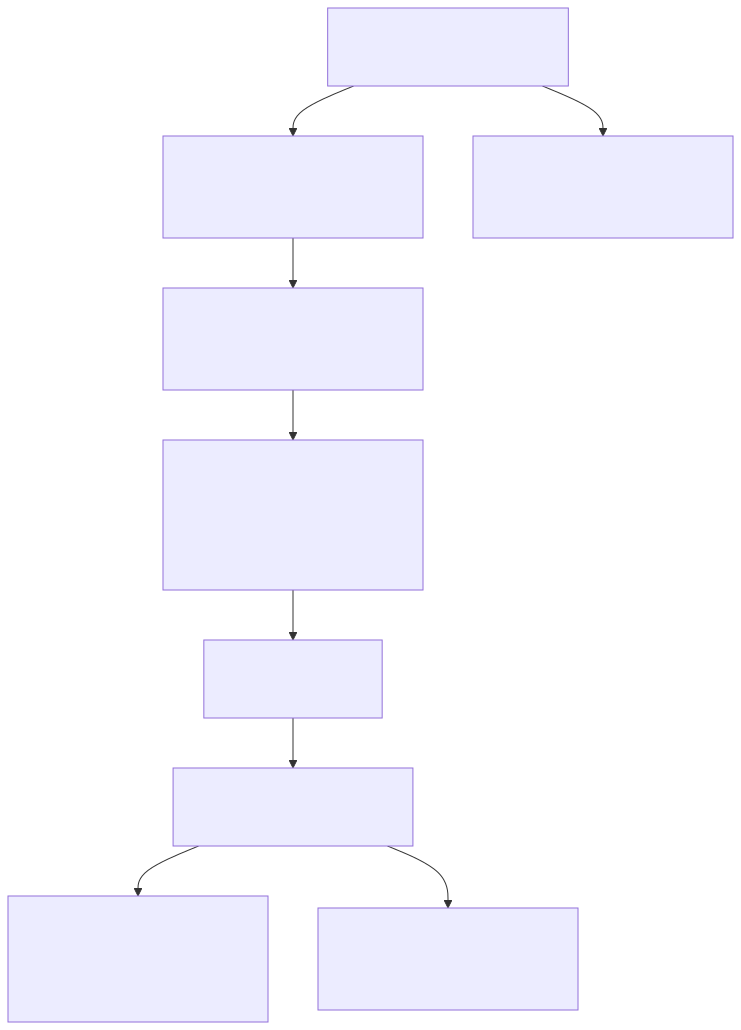
\includegraphics[width=\maxwidth,keepaspectratio,alt={Mermaid Diagram 1}]{0005-proof-of-relay/mermaid_1.png}}
\caption{Mermaid Diagram 1}
\end{figure}

\begin{enumerate}
\def\labelenumi{\arabic{enumi}.}
\item
  \codebubble{Ticket --sign--> VerifiedTicket}

  \begin{itemize}
  \item
    Pre-conditions:

    \begin{itemize}
    \tightlist
    \item
      Ticket MUST include all mandatory fields and satisfy bounds
      (amount ≤ 10\^{}25; index ≤ 2\^{}48; index\_offset ≥ 1;
      channel\_epoch ≤ 2\^{}24).
    \end{itemize}
  \item
    Post-conditions:

    \begin{itemize}
    \tightlist
    \item
      A valid ECDSA signature over
      \codebubble{get\_hash(domainSeparator)} is attached.
    \end{itemize}
  \end{itemize}
\item
  \codebubble{Ticket --verify(issuer, domainSeparator)--> VerifiedTicket}

  \begin{itemize}
  \tightlist
  \item
    MUST recover \codebubble{issuer} from \codebubble{signature} over
    \codebubble{get\_hash(domainSeparator)}.
  \item
    On failure, verification MUST be rejected.
  \end{itemize}
\item
  \codebubble{VerifiedTicket --into\_unacknowledged(own\_key)--> UnacknowledgedTicket}

  \begin{itemize}
  \tightlist
  \item
    Binds the recipient's PoR half-key. No additional checks REQUIRED.
  \end{itemize}
\item
  \codebubble{UnacknowledgedTicket --acknowledge(ack\_key)--> AcknowledgedTicket}

  \begin{itemize}
  \tightlist
  \item
    Compute \codebubble{Response = combine(own\_key, ack\_key)}.
  \item
    The derived challenge \codebubble{Response.to\_challenge()} MUST
    equal \codebubble{ticket.challenge}.
  \item
    On mismatch, the transition MUST fail with
    \codebubble{InvalidChallenge} and the ticket MUST remain
    unacknowledged.
  \end{itemize}
\item
  \codebubble{AcknowledgedTicket(Untouched) --into\_redeemable(chain\_keypair, domainSeparator)--> RedeemableTicket}

  \begin{itemize}
  \tightlist
  \item
    The caller (redeemer) MUST NOT be the ticket issuer (Loopback
    prevention).
  \item
    Derive VRF parameters over
    \codebubble{(verified\_hash, redeemer, domainSeparator)}.
  \item
    The resulting RedeemableTicket MAY be submitted on-chain if winning
    (see §3).
  \end{itemize}
\item
  \codebubble{AcknowledgedTicket(Untouched) --into\_transferable(chain\_keypair, domainSeparator)--> TransferableWinningTicket}

  \begin{itemize}
  \tightlist
  \item
    Equivalent to \codebubble{into\_redeemable} followed by conversion
    to transferable form; retains VRF and response.
  \end{itemize}
\item
  \codebubble{TransferableWinningTicket --into\_redeemable(expected\_issuer, domainSeparator)--> RedeemableTicket}

  \begin{itemize}
  \tightlist
  \item
    MUST verify: \codebubble{signer == expected\_issuer} and the
    embedded signature over \codebubble{get\_hash(domainSeparator)}.
  \item
    MUST recompute ``win'' locally (see §3). On failure, MUST reject.
  \end{itemize}
\item
  \codebubble{VerifiedTicket --leak()--> Ticket}

  \begin{itemize}
  \tightlist
  \item
    Debug/escape hatch only. Implementations SHOULD avoid downgrading
    state in production flows.
  \end{itemize}
\end{enumerate}

\subsection{9. Appendix 3}\label{appendix-3}

Domain separator (\codebubble{dst}) for the current implementation (in
Solidity) is derived as:

\begin{codebubbleenv}
domainSeparator = keccak256(
  abi.encode(
    keccak256("EIP712Domain(string name,string version,uint256 chainId,address verifyingContract)"),
    keccak256(bytes("HoprChannels")),
    keccak256(bytes(VERSION)),
    chainId,
    address(this)
  )
)
\end{codebubbleenv}

\subsection{10. References}\label{references}

{[}01{]} Bradner, S. (1997).
\href{https://datatracker.ietf.org/doc/html/rfc2119}{Key words for use
in RFCs to Indicate Requirement Levels}. \emph{IETF RFC 2119}.

{[}02{]} Faz-Hernandez, A., et al.~(2023).
\href{https://www.rfc-editor.org/rfc/rfc9380.html}{Hashing to Elliptic
Curves}. \emph{IETF RFC 9380}.
